\chapter{Smith Waterman}
\section{The scoring model. The BLOSUM62 matrix}
When two sequences are compared the question that needs an answer is:\\How much they are similar?\\
 The scoring model that we want to consider is based on the use of\textit{ Substitutional matrix} and \textit{Gap penalty} in the chosen alignment algorithm.\\Substitutional matrix and Gap penalty have been created to evaluate different mutation processes that can occur (as we can see in Fig. \ref{sw1} ).\\ 
 With a Substitutional matrix we consider amino acids \textit{matching} and \textit{substitutions}. While with the Gap penalty we consider amino acid \textit{insertions} or \textit{deletions}.
               \begin{figure}[h!]
               	\centering
               	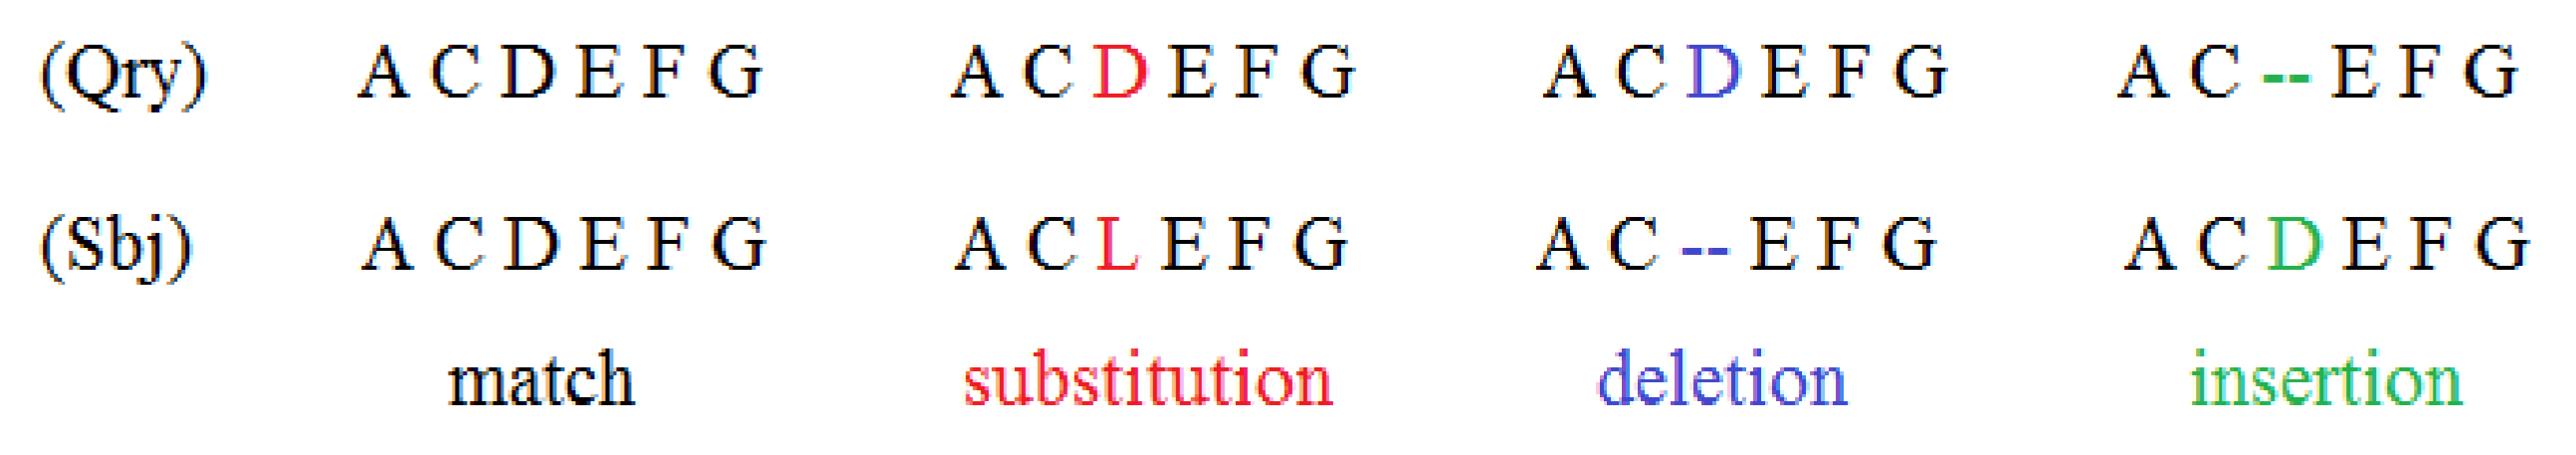
\includegraphics[width=0.85\textwidth]{imm/sw/sw1.png} 	\caption{Alignments with matching, substitution, insertion and deletion.
               		} 
               	\label{sw1}
               \end{figure}
 
 
 
 The BLOSUM62 matrix was introduced in 1992 by Henikoff \& Henikoff \cite{sw-blosum} to give a score for substitution in the amino acid sequence comparisons.
  matrix assigns to each pair of AAs (amino acids), a value that indicates the degree of similarity.
 A positive value in the matrix (Fig. \ref{blosum62}) means that the two amino acids are similar and they are frequently exchanged each other. 
\begin{figure}[h!]
     	\centering
     	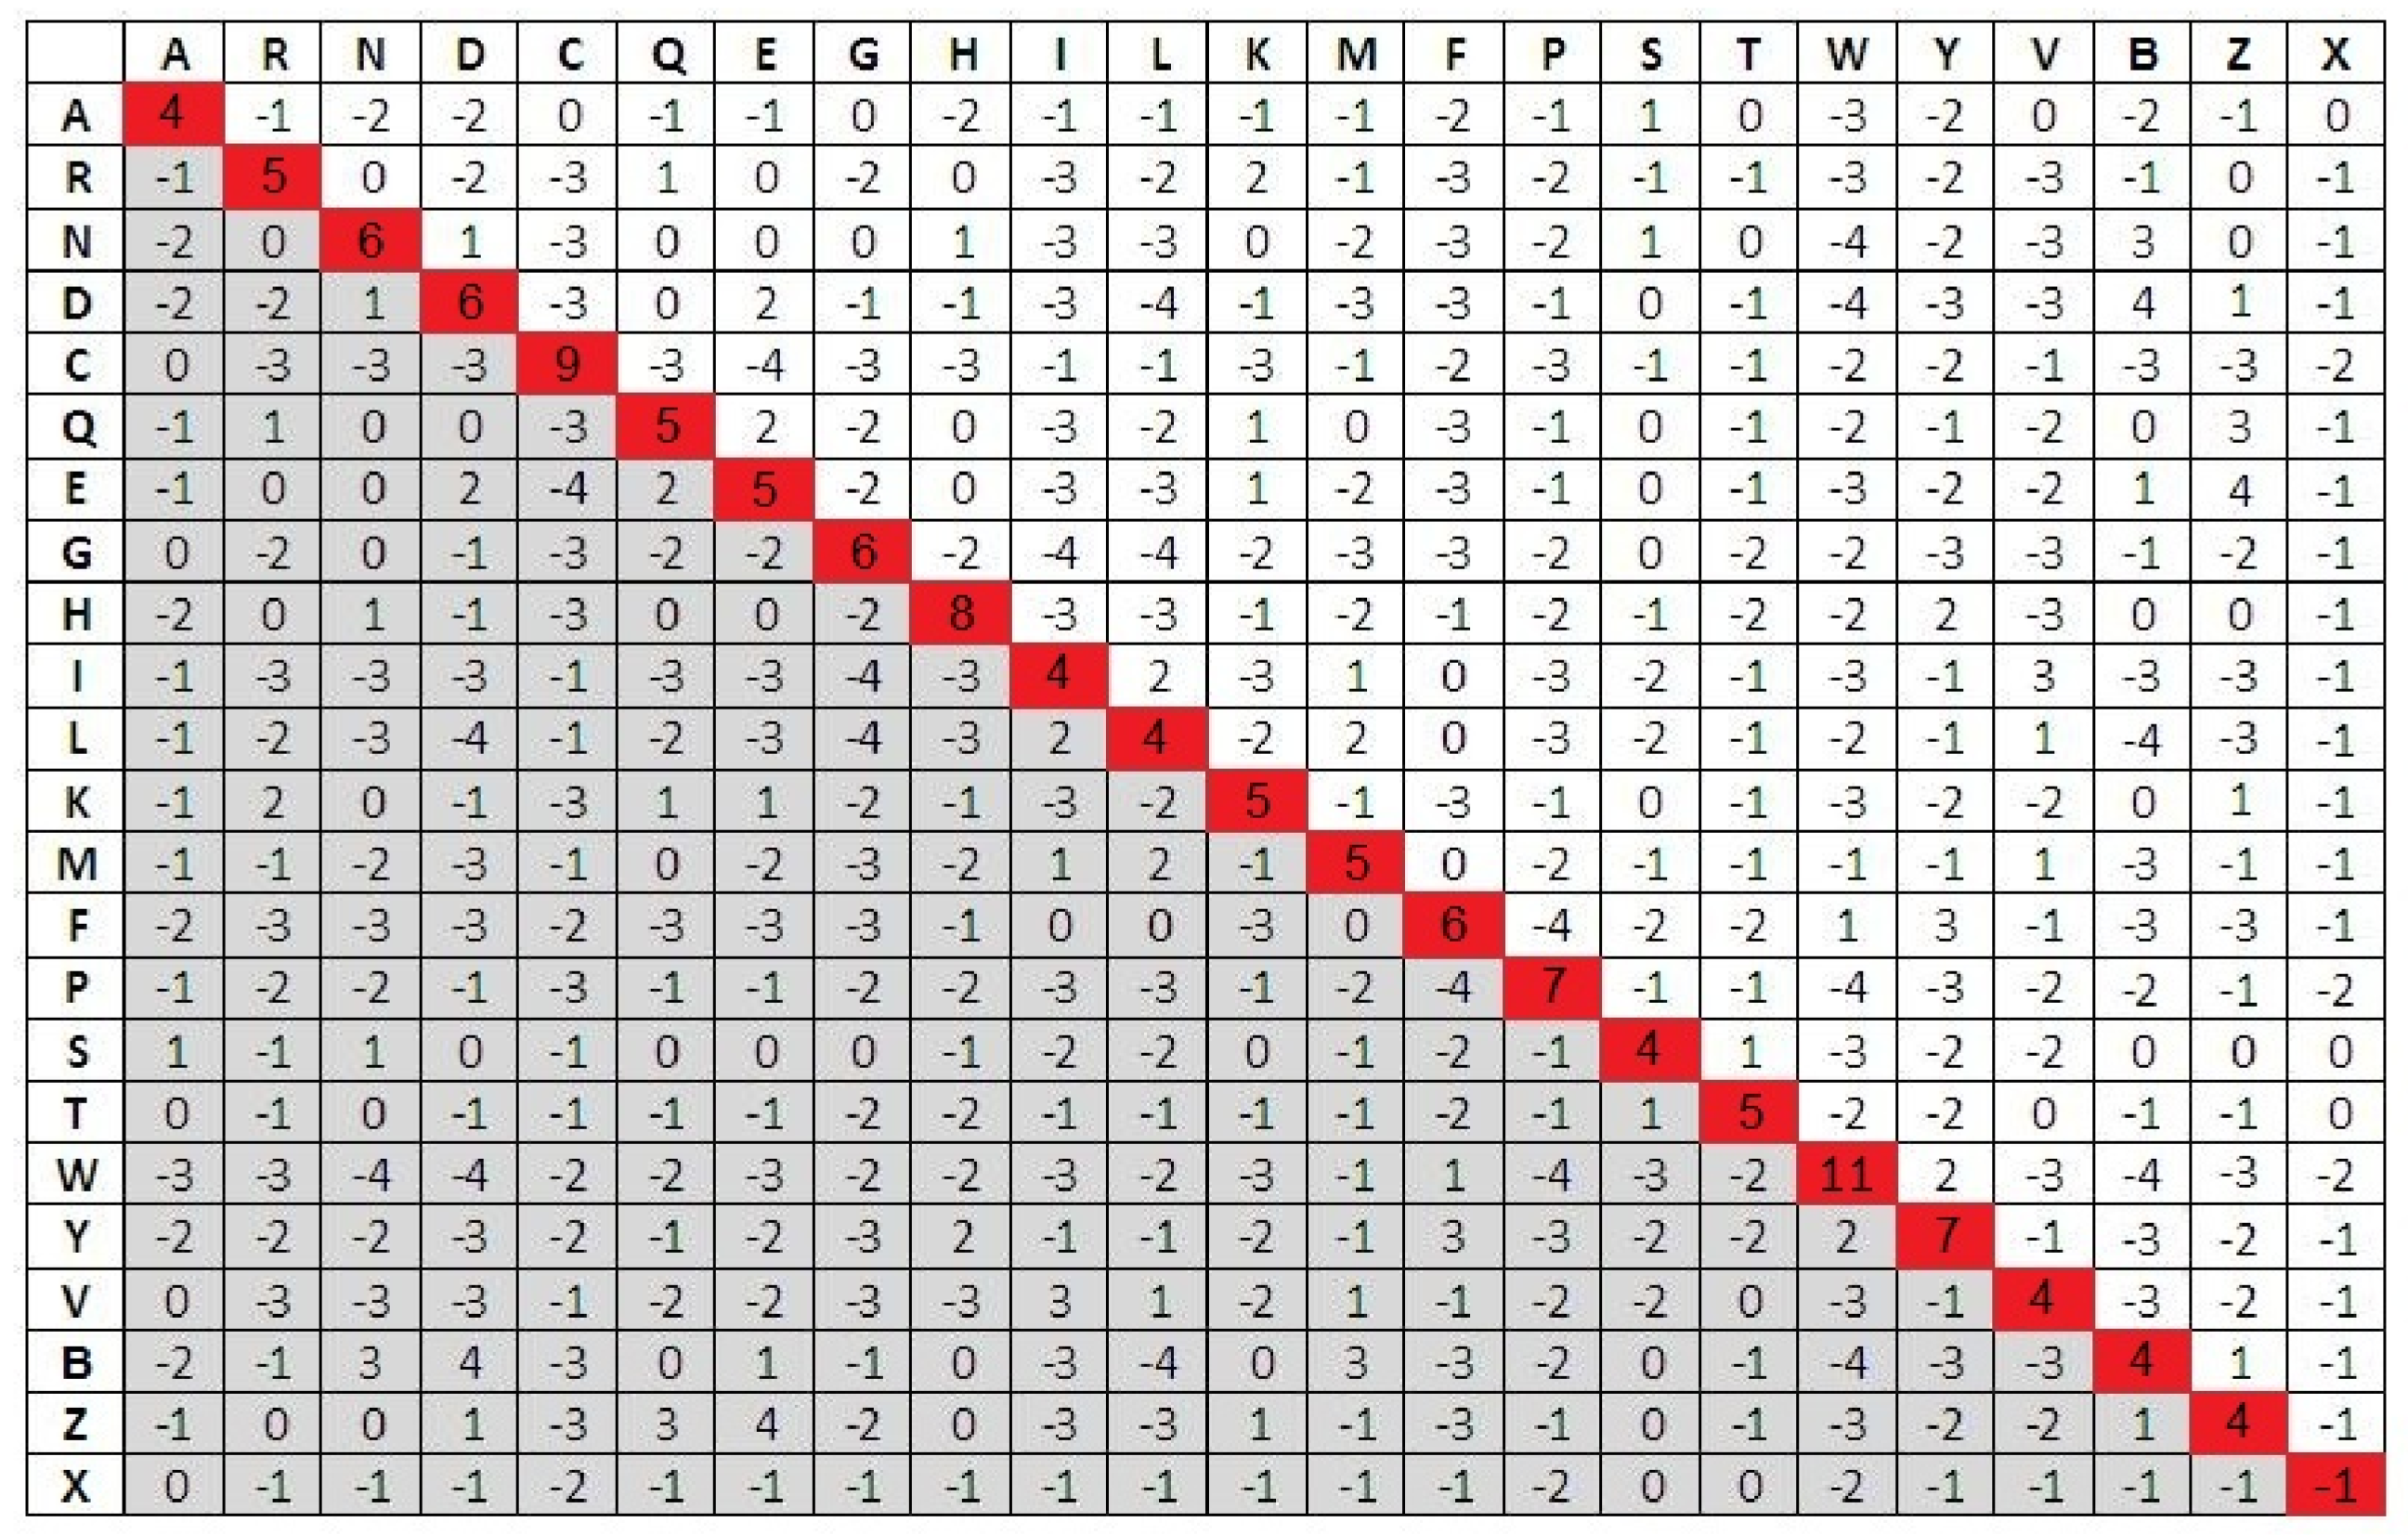
\includegraphics[width=0.85\textwidth]{imm/sw/blosum62.png} 	\caption{The BLOSUM62 substitution matrix.} 
     	\label{blosum62}
\end{figure}
\clearpage
\section{Smith-Waterman Local alignment method	}
Smith and Waterman in 1981 described a Local alignment method whose aim  is to find common regions between two protein (Qry, Sbj) through calculation of similarity score. \\
This algorithm can be substantially described in three steps:
\begin{enumerate}
	\item  \textbf{Initialization}; first row F(i,0) and first column F(0,j) are initialized to 0. Since it is always better to start a new local alignment instead of extend alignments that have got a negative score.
	 \item \textbf{Score matrix filling}; the score is calculated with the Eq. (\ref{sw_eq}) cell by cell.\\
	 \begin{equation}\label{sw_eq}
	 F(i,j) = max \begin{cases}
	
	 0 & \\
	  F(i-1,j-1) + s(Qry(i),Sbj(j))\qquad &\\
	   F(i-1,j)-d &\\
	   F(i,j-1)-d &
	 \end{cases} 
	 \end{equation}
	  if the first term '0' in the equation is selected as max it means that the previous alignment is ended or not alignment is possible. \\Since this algorithm evaluates local alignments, in this matrix there are not negative score.
	 
	
\end{enumerate}

\section{Simulation and Test}
The testbench of this architecture is divided in 3 phases:
\begin{enumerate}
	\item \textbf{Phase 1-sub\_matr\_and\_gap\_load }:  configure the systolic array trough the loading of all the storage registers with values coming from the substitutional matrix and gap files.\\
	\item  \textbf{Phase 2-s\_w\_computation}: It starts when the configuration process is terminated and reads from the DB file the Sbj id number and the associated amino acids sequence. In this phase we compute the S-W algorithm. This process is ended when all the database is scanned.\\
	\item \textbf{Phase 3-output\_writing}: It checks, in each clock cycle, if the stored Sbj id is changed. If the Sbj id is different, this process will write on the output file the n. of Sbj id and the associated Maximum Alignment Score.
	
	
	
\end{enumerate}
\begin{figure}[h!]
	\centering
	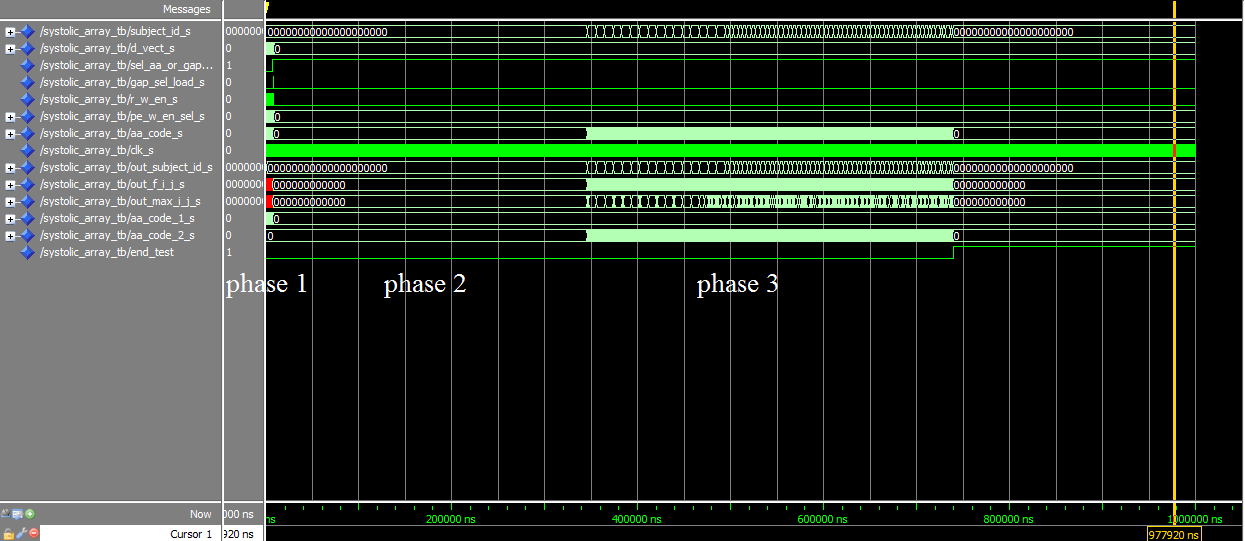
\includegraphics[width=\textwidth]{imm/sw/tb_systolic_array_phases.png} 	\caption{Phases of the testbench} 
	\label{tb_sw}
\end{figure}

\begin{figure}[h!]
	\centering
	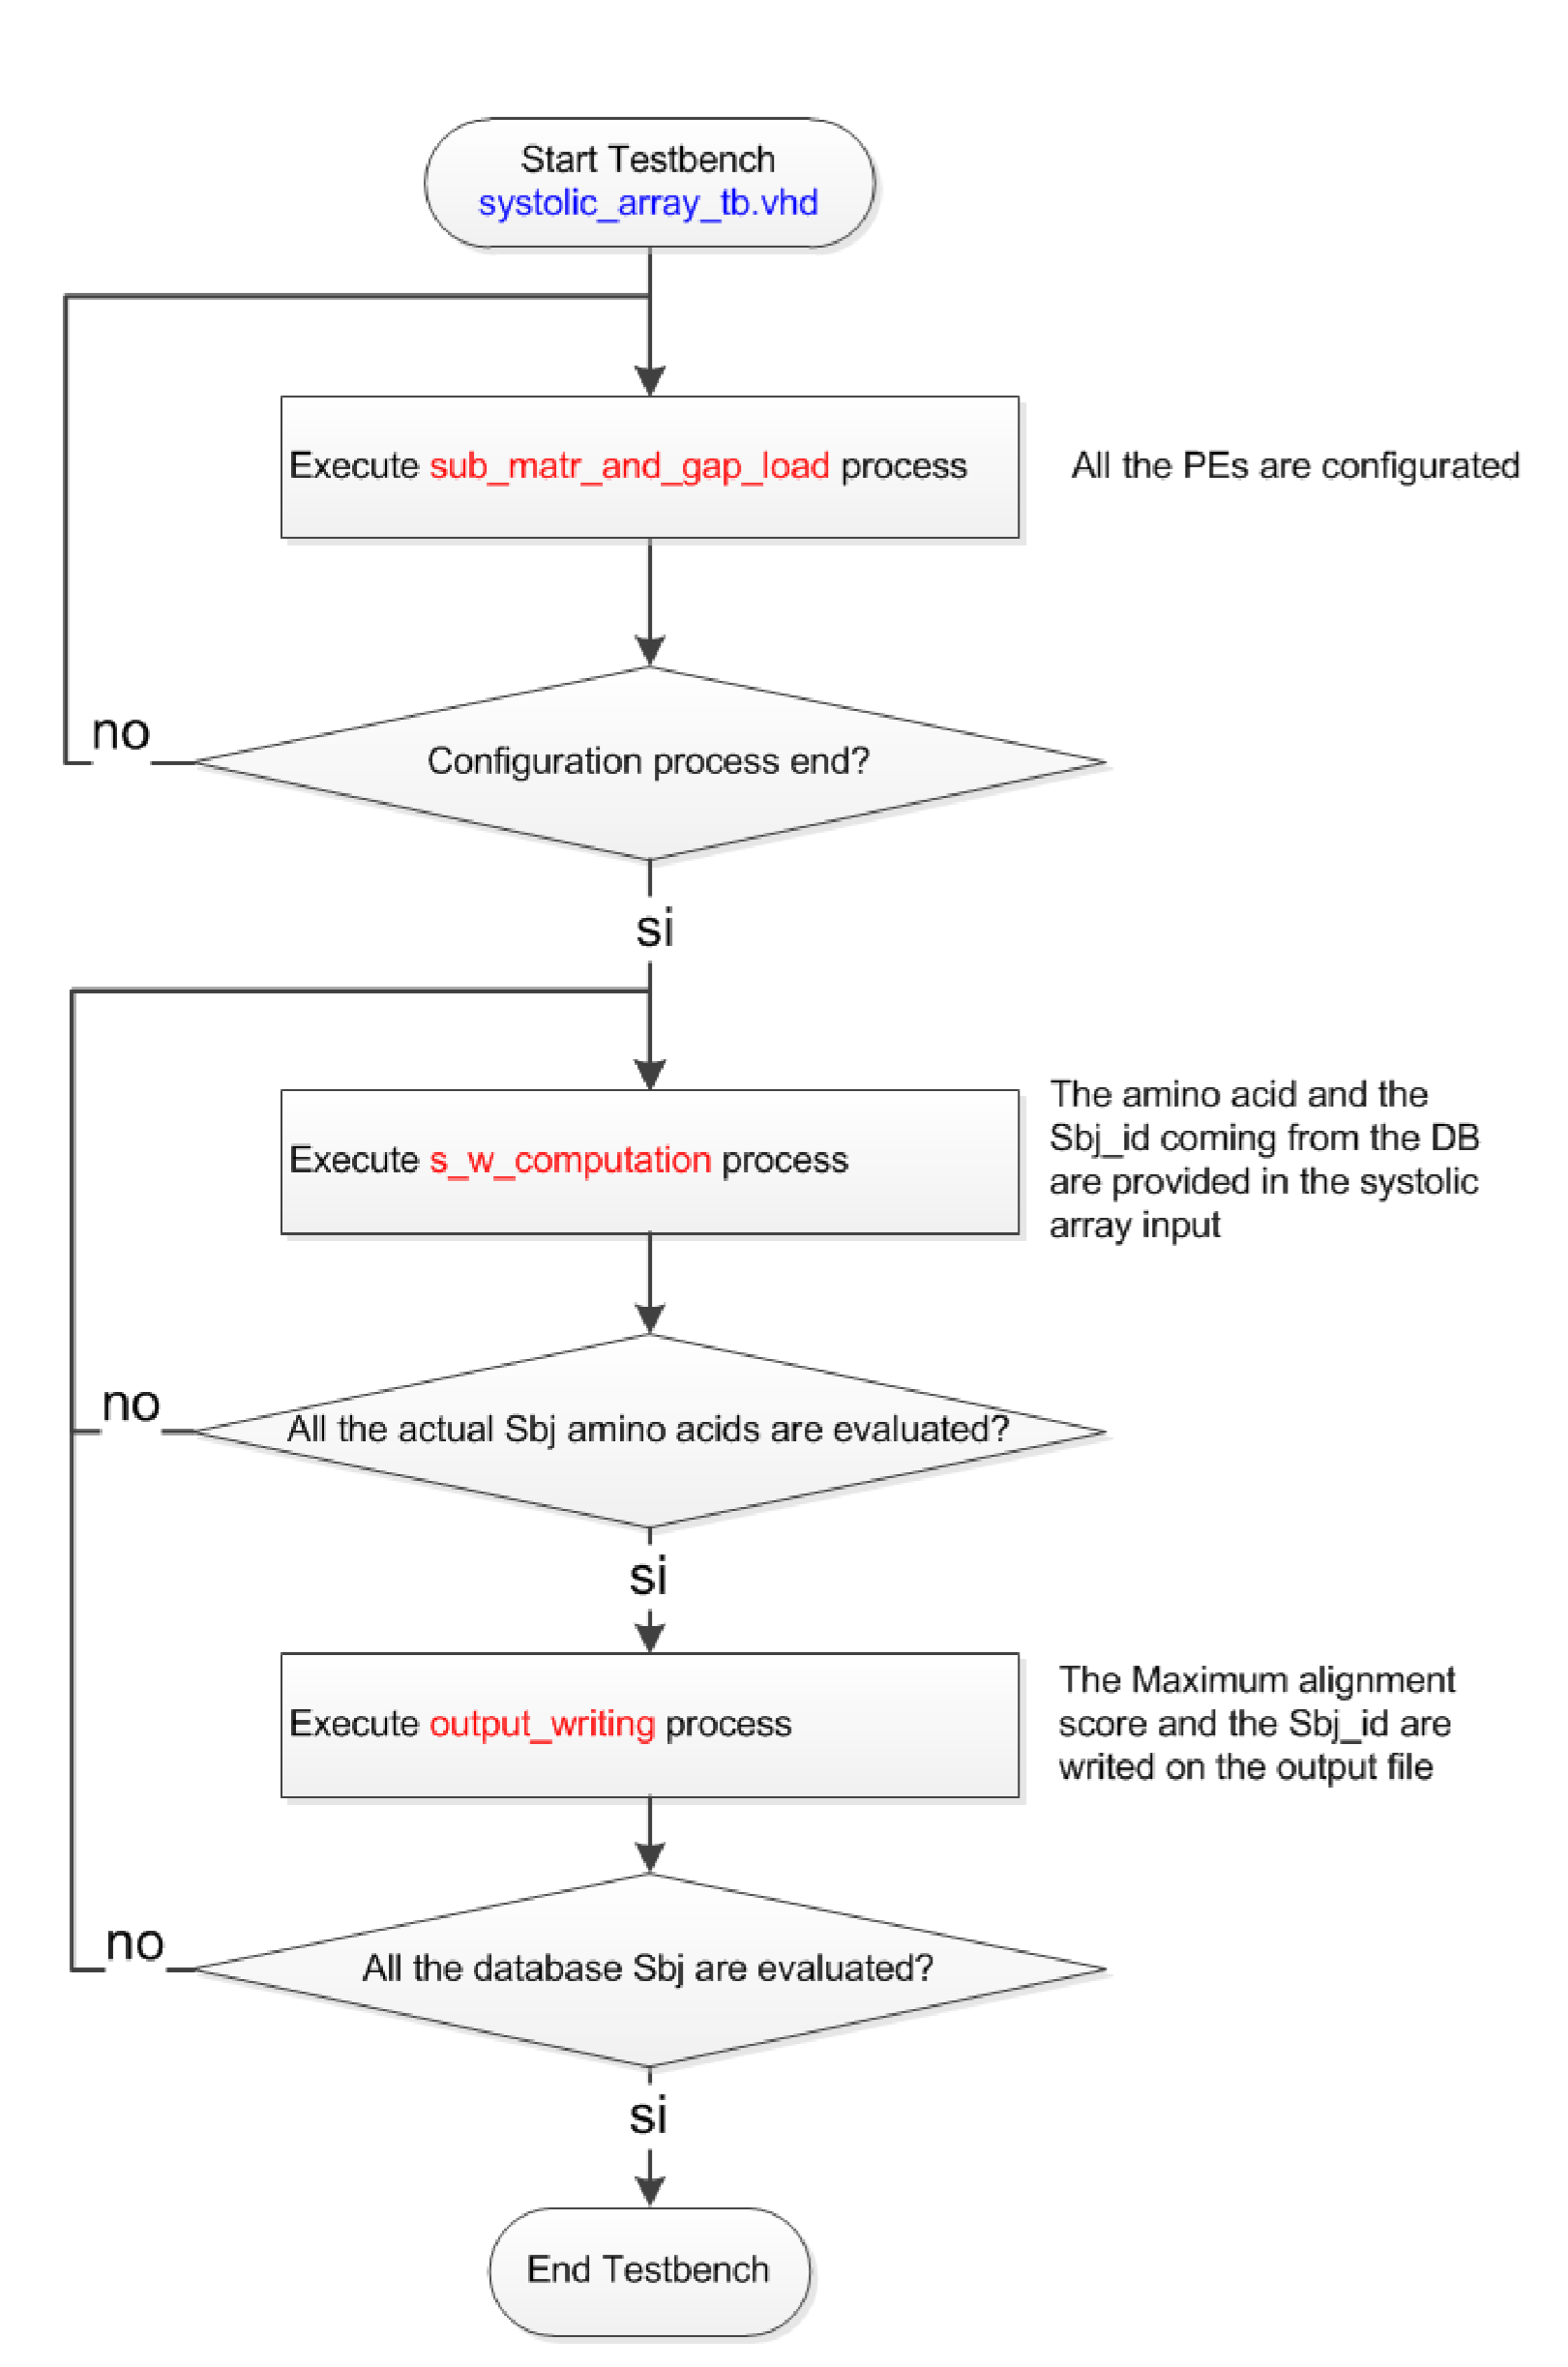
\includegraphics[width=0.7\textwidth]{imm/sw/tb_flow.png} 	\caption{Main flow chart of \textit{systolic\_array\_tb.vhd} testbench. In blue the testbench name, in red the processes name} 
	\label{tb_sw_flow}
\end{figure}

\clearpage
\newpage

\subsection{Phase 1-sub\_matr\_and\_gap\_load }
\begin{figure}[h!]
	\centering
	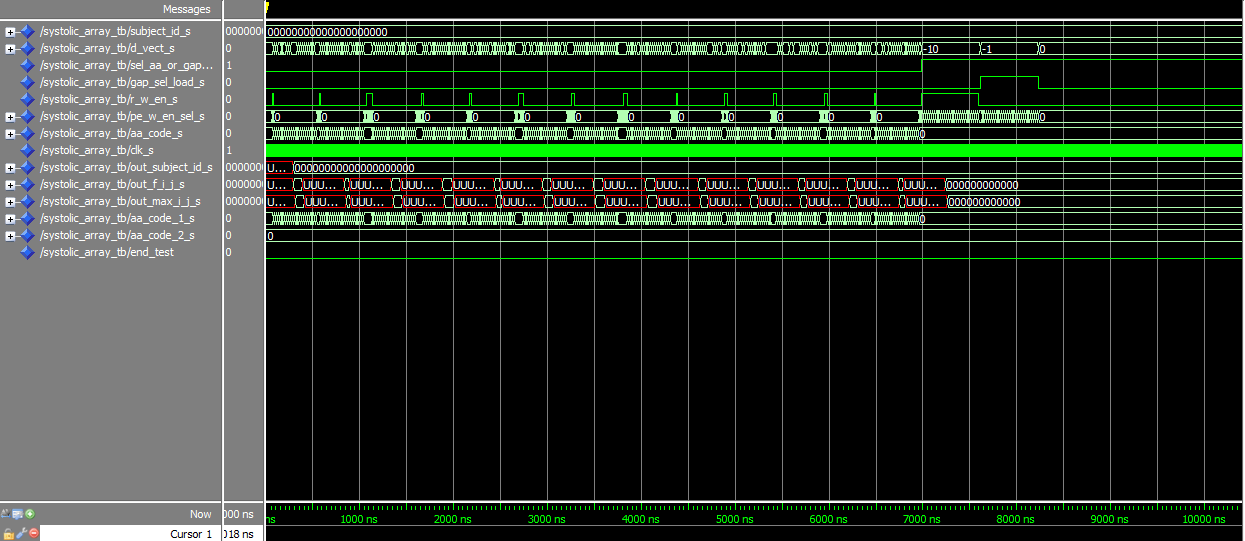
\includegraphics[width=\textwidth]{imm/sw/configuration_phase.png} 	\caption{Phase 1 of the testbench} 
	\label{tb_sw_1}
\end{figure}